\section{Исследовательская часть}

\subsection{Технические характеристики}

\begin{itemize}
	\item процессор: 13th Gen Intel(R) Core(TM) i5-13500H (16 ядер) @ 4.70ГГц;
	\item оперативная память: 16 ГБайт;
	\item операционная система: EndeavourOS x86\_64.
\end{itemize}

При замерах ноутбук был включен в сеть и был нагружен только системными приложениями.

\subsection{Результаты проводимых исследований}

В ходе исследования сравнивается время, необходимое на поиск пути.

Результаты исследования изображены на рисунке~\ref{plt:graphic1}.

В процессе исследования для алгоритма муравьиного использовался промежуток времени: 200 дней.

\begin{figure}[h]
	\centering
	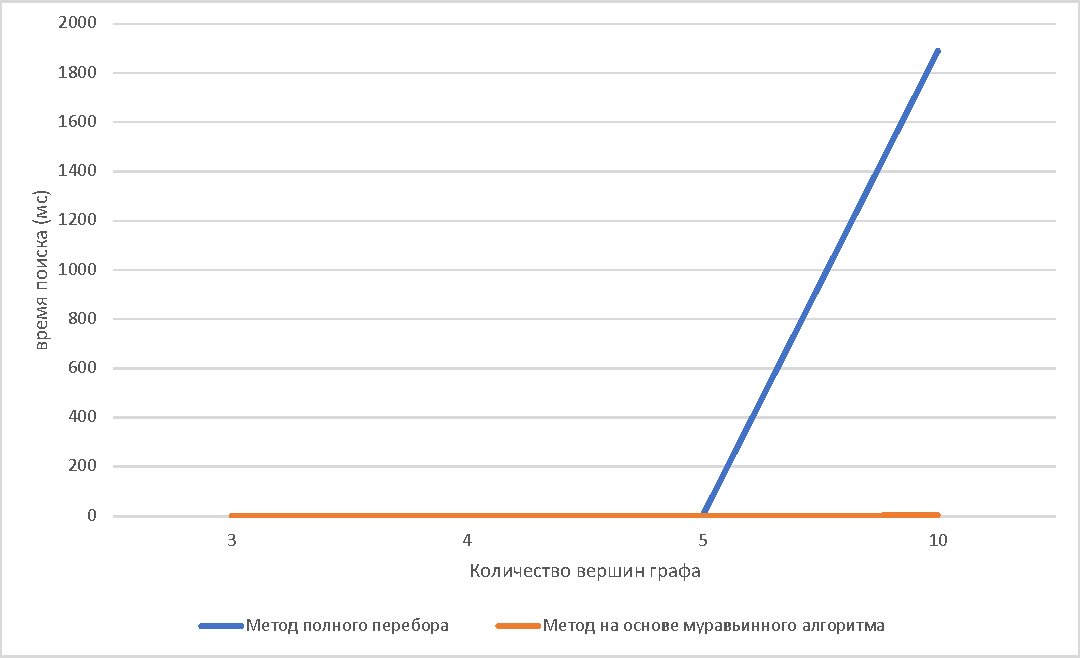
\includegraphics[height=0.3\textheight]{imgs/measuring.pdf}
	\caption{Сравнение временных затрат на поиск пути}
	\label{plt:graphic1}
\end{figure}

\subsection{Параметризация}

Параметризация проведена на классе данных состоящем из трех графов ---~\ref{eq:kd1}--\ref{eq:kd3}. Алгоритм запущен для набора значений $\alpha, \rho \in (0, 1), days = \{1, 3, 5, 10, 50, 100, 300, 500\}, e = \{0.5, 1, 2\}$.

Полученная таблица значений в ходе параметризации состоит из колонок:
\begin{itemize}[label=---]
	\item $\alpha$ --- коэффициент жадности;
	\item $\rho$ --- коэффициент испарения;
	\item \textit{days} --- количество дней жизни колонии муравьев;
	\item \textit{Result} --- эталонный результат, полученный методом полного перебора для проведения данного исследования;
	\item \textit{Mistake} --- показатель качества решения, полученный путем разности эталонного решения и решения методом на основе муравьиного алгоритма.
\end{itemize}

Цель параметризации --- определить комбинацию параметров, которые позволяют решить задачу наилучшим образом для выбранного графа. Качество решения зависит от количества дней и погрешности измерений.

\subsubsection{Класс данных}
Класс данных состоит из 3 матриц смежности размером 10 элементов (см. таблицы~\ref{eq:kd1}--\ref{eq:kd3}).

\begin{equation}
    \label{eq:kd1}
	K_{1} = \begin{pmatrix}
0 & 45 & 0 & 2 & 39 & 3 & 46 & 87 & 95 & 39  \\
45 & 0 & 71 & 54 & 42 & 69 & 76 & 27 & 10 & 66  \\
0 & 71 & 0 & 51 & 10 & 3 & 9 & 42 & 22 & 72  \\
2 & 54 & 51 & 0 & 98 & 6 & 6 & 45 & 62 & 78  \\
39 & 42 & 10 & 98 & 0 & 21 & 78 & 67 & 65 & 64  \\
3 & 69 & 3 & 6 & 21 & 0 & 64 & 37 & 44 & 48  \\
46 & 76 & 9 & 6 & 78 & 64 & 0 & 55 & 65 & 88  \\
87 & 27 & 42 & 45 & 67 & 37 & 55 & 0 & 23 & 70  \\
95 & 10 & 22 & 62 & 65 & 44 & 65 & 23 & 0 & 78  \\
39 & 66 & 72 & 78 & 64 & 48 & 88 & 70 & 78 &  0 \\
	\end{pmatrix}
\end{equation}


\begin{equation}
	\label{eq:kd2}
	K_{2} = \begin{pmatrix}
0 & 85 & 18 & 25 & 42 & 97 & 77 & 80 & 69 & 2 \\
85 & 0 & 18 & 88 & 1 & 26 & 55 & 11 & 19 & 28 \\
18 & 18 & 0 & 51 & 44 & 36 & 49 & 54 & 83 & 61 \\
25 & 88 & 51 & 0 & 27 & 22 & 45 & 71 & 7 & 11 \\
42 & 1 & 44 & 27 & 0 & 96 & 80 & 53 & 16 & 5 \\
97 & 26 & 36 & 22 & 96 & 0 & 89 & 7 & 9 & 16 \\
77 & 55 & 49 & 45 & 80 & 89 & 0 & 68 & 95 & 12 \\
80 & 11 & 54 & 71 & 53 & 7 & 68 & 0 & 91 & 3 \\
69 & 19 & 83 & 7 & 16 & 9 & 95 & 91 & 0 & 48 \\
2 & 28 & 61 & 11 & 5 & 16 & 12 & 3 & 48 & 0	 \\
	\end{pmatrix}
\end{equation}

\begin{equation}
	\label{eq:kd3}
	K_{3} = \begin{pmatrix}
0 & 20 & 45 & 89 & 91 & 99 & 91 & 58 & 95 & 44 \\
20 & 0 & 29 & 62 & 59 & 8 & 83 & 38 & 35 & 21 \\
45 & 29 & 0 & 11 & 58 & 1 & 2 & 3 & 5 & 47 \\
89 & 62 & 11 & 0 & 57 & 23 & 82 & 48 & 9 & 71 \\
91 & 59 & 58 & 57 & 0 & 53 & 72 & 81 & 86 & 12 \\
99 & 8 & 1 & 23 & 53 & 0 & 16 & 14 & 13 & 30 \\
91 & 83 & 2 & 82 & 72 & 16 & 0 & 7 & 10 & 25 \\
58 & 38 & 3 & 48 & 81 & 14 & 7 & 0 & 9 & 46 \\
95 & 35 & 5 & 9 & 86 & 13 & 10 & 9 & 0 & 54 \\
44 & 21 & 47 & 71 & 12 & 30 & 25 & 46 & 54 & 0 \\
	\end{pmatrix}
\end{equation}

Результаты параметризации представлены в приложении А.